\documentclass{standalone}
\usepackage{tikz}

\begin{document}
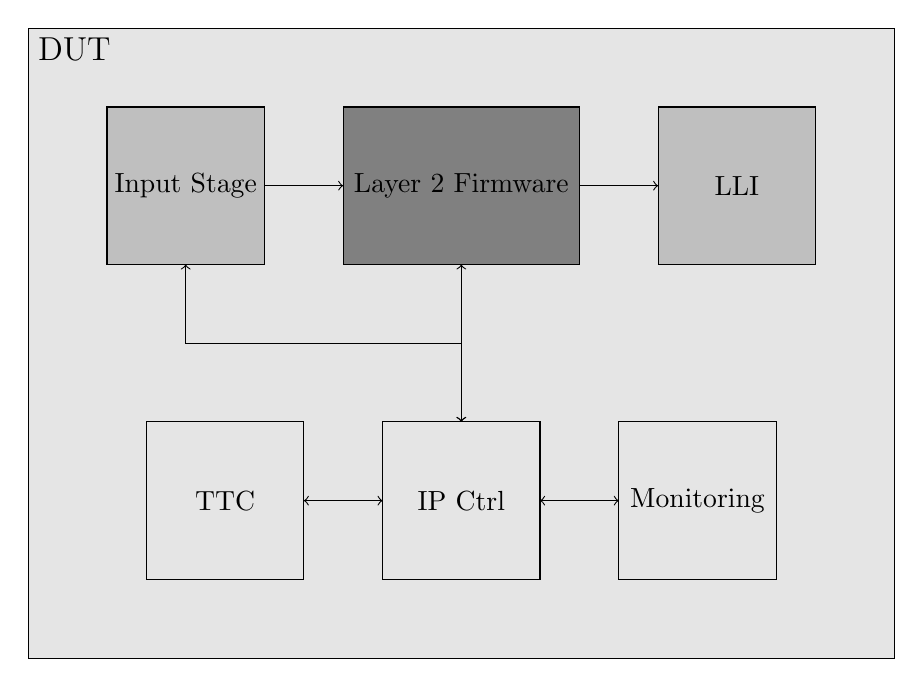
\begin{tikzpicture}[]

% Background rectangle with borders (larger)
\draw[fill=gray!20] (5,-5) rectangle (16,3);

% "DUT" at the top left of the background rectangle
\node[anchor=north west, font=\large] at (5,3) {DUT};

\draw[fill=lightgray] (6,0) rectangle (8,2);
\node[align=center] at (7,1) {Input Stage};

% Arrow coming out of the 3rd block
\draw[->] (8,1) -- (9,1);

% 4th block: User Code Bypass (dashed border)
\draw[fill=gray] (9,0) rectangle (12,2);
\node[align=center] at (10.5,1) {Layer 2 Firmware};

% Arrow coming out of the 4th block
\draw[->] (12,1) -- (13,1);

\draw[fill=lightgray] (13,0) rectangle (15,2);
\node[align=center] at (14,1) {LLI};

\draw[] (6.5,-4) rectangle (8.5,-2);
\node[align=center] at (7.5,-3) {TTC};

% Arrow coming out of the 3rd block
\draw[<->] (8.5,-3) -- (9.5,-3);

% 4th block: User Code Bypass (dashed border)
\draw[] (9.5,-4) rectangle (11.5,-2);
\node[align=center] at (10.5,-3) {IP Ctrl};

\draw[<->] (10.5,-2) -- (10.5,-1) -- (7,-1) -- (7,0);
\draw[<->] (10.5,-2) -- (10.5,0);

% Arrow coming out of the 4th block
\draw[<->] (11.5,-3) -- (12.5,-3);

\draw[] (12.5,-4) rectangle (14.5,-2);
\node[align=center] at (13.5,-3) {Monitoring};

\end{tikzpicture}
\end{document}